\documentclass[letterpaper,11pt]{article}

\usepackage{geometry}
\usepackage{pslatex}
\usepackage{fancyhdr}
\usepackage{graphicx}
\usepackage{color}
\usepackage{tikz}
\usepackage{setspace}
\geometry{ margin = 1.0in }

\pagestyle{fancy}
\lhead{{\bf Lecture 30}}
\chead{{\bf CMPSC 465 Fall 2020}}
\rhead{{\bf Mingfu Shao}}

\setlength\parindent{0em}
\setlength\parskip{8pt}
%\setlength{\fboxsep}{6pt}

\usepackage{amsthm}
\newtheoremstyle{mytheorem}
  {\parskip} % Space above
  {0em} % Space below
  {} % Body font
  {} % Indent amount
  {\bfseries} % Theorem head font
  {.} % Punctuation after theorem head
  {.5em} % Space after theorem head
  {} % Theorem head spec (can be left empty, meaning `normal')

\theoremstyle{mytheorem}
\newtheorem{definition}{Definition}
\newtheorem{property}{Property}
\newtheorem{claim}{Claim}
\newtheorem{fact}{Fact}
\newtheorem{corollary}{Corollary}

% for algorithms
\newcommand{\aaa}[1]{\hspace{0.65cm}\parbox[t]{15.3cm}{#1}}
\newcommand{\aab}[1]{\hspace{1.15cm}\parbox[t]{15.0cm}{#1}}
\newcommand{\aac}[1]{\hspace{1.65cm}\parbox[t]{15.0cm}{#1}}
\newcommand{\aad}[1]{\hspace{2.15cm}\parbox[t]{15.0cm}{#1}}
\newcommand{\aae}[1]{\hspace{2.65cm}\parbox[t]{15.0cm}{#1}}
\newcommand{\aaf}[1]{\hspace{3.15cm}\parbox[t]{15.0cm}{#1}}
\newcommand{\aaA}[2]{\hspace{0.5cm} {\tikz[overlay] \draw (0.1, -0.1) -- (0.1, #1 * -1.5em + 0.6em);} \parbox[t]{15.0cm}{#2}}
\newcommand{\aaB}[2]{\hspace{1.0cm} {\tikz[overlay] \draw (0.1, -0.1) -- (0.1, #1 * -1.5em + 0.6em);} \parbox[t]{15.0cm}{#2}}
\newcommand{\aaC}[2]{\hspace{1.5cm} {\tikz[overlay] \draw (0.1, -0.1) -- (0.1, #1 * -1.5em + 0.6em);} \parbox[t]{15.0cm}{#2}}
\newcommand{\aaD}[2]{\hspace{2.0cm} {\tikz[overlay] \draw (0.1, -0.1) -- (0.1, #1 * -1.5em + 0.6em);} \parbox[t]{15.0cm}{#2}}
\newcommand{\aaE}[2]{\hspace{2.5cm} {\tikz[overlay] \draw (0.1, -0.1) -- (0.1, #1 * -1.5em + 0.6em);} \parbox[t]{15.0cm}{#2}}
\newcommand{\xxx}{\par\vspace{0.1cm}}

\begin{document}

\section*{Minimum Spanning Tree}

\subsection*{Tree and Spanning Tree}

A tree is an undirected graph that is connected and acyclic.
(``connected'' here means the graph consists of a single connected component.)
A tree $T = (V, E)$ always satisfies that $|E| = |V| - 1$.
In fact, any two of these three properties~(i.e., connected, acyclic, and $|E| = |V| - 1$)
implies the other one, formally stated below. Play with some examples
to fully understand these properties.

\begin{fact}\label{fact1}
Let $T = (V, E)$ be an undirected graph. The following statements are equivalent.
\vspace*{-\topsep}
\begin{enumerate}
\item $T$ is a tree.
\item $T$ is connected and acyclic.
\item $|E| = |V| - 1$ and $T$ is acyclic.
\item $|E| = |V| - 1$ and $T$ is connected.
\item There exists an unique path between every pair of vertices of $T$.
\end{enumerate}
\end{fact}

Let $G = (V,E)$ be an undirected graph.
We say tree $T = (V_1, E_1)$ is a \emph{spanning tree}
of $G$ if $V_1 = V$ and $E_1\subset E$.
As $T$ is a tree, clearly we have $|E_1| = |V_1| - 1 = |V| - 1$.
Note that a spanning tree is always w.r.t.\ a graph, i.e., we always
say a spanning tree of a graph. Note too, that for an undirected graph $G$, 
its spanning tree may not be unqiue. See Figure~\ref{fig:spanning}
for an example.  (Think: when an undirected graph has a unique spanning tree?)

\begin{figure}[h]
\centering{

\tikzset{every picture/.style={line width=0.75pt}} %set default line width to 0.75pt        

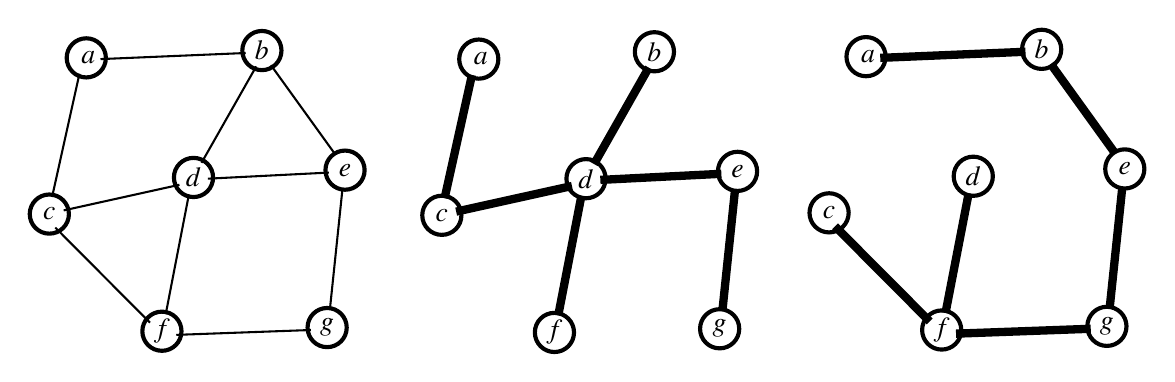
\begin{tikzpicture}[x=0.5pt,y=0.5pt,yscale=-1,xscale=1]
%uncomment if require: \path (0,290); %set diagram left start at 0, and has height of 290

%Straight Lines [id:da6859712806144006] 
\draw [color={rgb, 255:red, 0; green, 0; blue, 0 }  ,draw opacity=1 ][line width=0.75]    (185,39.17) -- (231.39,103.54) ;
%Straight Lines [id:da43828905709564314] 
\draw [color={rgb, 255:red, 0; green, 0; blue, 0 }  ,draw opacity=1 ][line width=0.75]    (116.55,234.06) -- (213.9,230.54) ;
%Straight Lines [id:da6385368954330931] 
\draw [color={rgb, 255:red, 0; green, 0; blue, 0 }  ,draw opacity=1 ][line width=0.75]    (29.1,156.46) -- (97.54,225.24) ;
%Straight Lines [id:da061278223687582845] 
\draw [color={rgb, 255:red, 0; green, 0; blue, 0 }  ,draw opacity=1 ][line width=0.75]    (35.18,144.11) -- (118.84,125.59) ;
%Straight Lines [id:da125058897644165] 
\draw [color={rgb, 255:red, 0; green, 0; blue, 0 }  ,draw opacity=1 ][line width=0.75]    (46.59,45.34) -- (26.81,134.41) ;
%Straight Lines [id:da7561477389708726] 
\draw [color={rgb, 255:red, 0; green, 0; blue, 0 }  ,draw opacity=1 ][line width=0.75]    (61.8,34.76) -- (166.75,30.35) ;
%Straight Lines [id:da8045438090716241] 
\draw [color={rgb, 255:red, 0; green, 0; blue, 0 }  ,draw opacity=1 ][line width=0.75]    (174.35,40.05) -- (134.81,109.72) ;
%Straight Lines [id:da7384444755679203] 
\draw [color={rgb, 255:red, 0; green, 0; blue, 0 }  ,draw opacity=1 ][line width=0.75]    (125.68,132.65) -- (108.95,219.07) ;
%Straight Lines [id:da7781378597799559] 
\draw [color={rgb, 255:red, 0; green, 0; blue, 0 }  ,draw opacity=1 ][line width=0.75]    (236.71,128.24) -- (227.59,215.54) ;
%Straight Lines [id:da6283012441188964] 
\draw [color={rgb, 255:red, 0; green, 0; blue, 0 }  ,draw opacity=1 ][line width=0.75]    (226.83,116.77) -- (139.37,121.18) ;
%Straight Lines [id:da438892015392218] 
\draw [color={rgb, 255:red, 0; green, 0; blue, 0 }  ,draw opacity=1 ][line width=3]    (318.85,144.99) -- (402.51,126.47) ;
%Straight Lines [id:da8359945945218459] 
\draw [color={rgb, 255:red, 0; green, 0; blue, 0 }  ,draw opacity=1 ][line width=3]    (330.26,46.22) -- (310.48,135.29) ;
%Straight Lines [id:da21420370300632352] 
\draw [color={rgb, 255:red, 0; green, 0; blue, 0 }  ,draw opacity=1 ][line width=3]    (458.02,40.93) -- (418.48,110.6) ;
%Straight Lines [id:da9239671202801586] 
\draw [color={rgb, 255:red, 0; green, 0; blue, 0 }  ,draw opacity=1 ][line width=3]    (409.35,133.53) -- (392.62,219.95) ;
%Straight Lines [id:da821215549767216] 
\draw [color={rgb, 255:red, 0; green, 0; blue, 0 }  ,draw opacity=1 ][line width=3]    (520.38,129.12) -- (511.26,216.43) ;
%Straight Lines [id:da9218980242104106] 
\draw [color={rgb, 255:red, 0; green, 0; blue, 0 }  ,draw opacity=1 ][line width=3]    (510.5,117.65) -- (423.04,122.06) ;
%Straight Lines [id:da35247521934474646] 
\draw [color={rgb, 255:red, 0; green, 0; blue, 0 }  ,draw opacity=1 ][line width=3]    (748.54,38.28) -- (794.93,102.66) ;
%Straight Lines [id:da7944029026500893] 
\draw [color={rgb, 255:red, 0; green, 0; blue, 0 }  ,draw opacity=1 ][line width=3]    (680.09,233.18) -- (777.44,229.65) ;
%Straight Lines [id:da39283588857656926] 
\draw [color={rgb, 255:red, 0; green, 0; blue, 0 }  ,draw opacity=1 ][line width=3]    (592.63,155.57) -- (661.08,224.36) ;
%Straight Lines [id:da24731320696047454] 
\draw [color={rgb, 255:red, 0; green, 0; blue, 0 }  ,draw opacity=1 ][line width=3]    (625.33,33.87) -- (730.28,29.46) ;
%Straight Lines [id:da24545478407911292] 
\draw [color={rgb, 255:red, 0; green, 0; blue, 0 }  ,draw opacity=1 ][line width=3]    (689.22,131.76) -- (672.49,218.19) ;
%Straight Lines [id:da379919078999982] 
\draw [color={rgb, 255:red, 0; green, 0; blue, 0 }  ,draw opacity=1 ][line width=3]    (800.25,127.35) -- (791.12,214.66) ;

% Text Node
\draw  [line width=1.5]   (238.52, 115.01) circle [x radius= 14.15, y radius= 14.15]   ;
\draw (238.52,115.01) node   [align=left] {$\displaystyle e$};
% Text Node
\draw  [line width=1.5]   (51.52, 33.87) circle [x radius= 14.15, y radius= 14.15]   ;
\draw (46.02,33.87) node [anchor=west] [inner sep=0.75pt]   [align=left] {$\displaystyle a$};
% Text Node
\draw  [line width=1.5]   (178.44, 28.58) circle [x radius= 14.15, y radius= 14.15]   ;
\draw (178.44,28.58) node   [align=left] {$\displaystyle b$};
% Text Node
\draw  [line width=1.5]   (24.82, 146.76) circle [x radius= 14.15, y radius= 14.15]   ;
\draw (24.82,146.76) node   [align=left] {$\displaystyle c$};
% Text Node
\draw  [line width=1.5]   (129.01, 120.3) circle [x radius= 14.15, y radius= 14.15]   ;
\draw (129.01,120.3) node   [align=left] {$\displaystyle d$};
% Text Node
\draw  [line width=1.5]   (106.19, 231.42) circle [x radius= 14.15, y radius= 14.15]   ;
\draw (106.19,231.42) node   [align=left] {$\displaystyle f$};
% Text Node
\draw  [line width=1.5]   (225.59, 228.77) circle [x radius= 14.15, y radius= 14.15]   ;
\draw (225.59,228.77) node   [align=left] {$\displaystyle g$};
% Text Node
\draw  [line width=1.5]   (522.19, 115.89) circle [x radius= 14.15, y radius= 14.15]   ;
\draw (522.19,115.89) node   [align=left] {$\displaystyle e$};
% Text Node
\draw  [line width=1.5]   (335.19, 34.76) circle [x radius= 14.15, y radius= 14.15]   ;
\draw (329.69,34.76) node [anchor=west] [inner sep=0.75pt]   [align=left] {$\displaystyle a$};
% Text Node
\draw  [line width=1.5]   (462.11, 29.46) circle [x radius= 14.15, y radius= 14.15]   ;
\draw (462.11,29.46) node   [align=left] {$\displaystyle b$};
% Text Node
\draw  [line width=1.5]   (308.49, 147.64) circle [x radius= 14.15, y radius= 14.15]   ;
\draw (308.49,147.64) node   [align=left] {$\displaystyle c$};
% Text Node
\draw  [line width=1.5]   (412.68, 121.18) circle [x radius= 14.15, y radius= 14.15]   ;
\draw (412.68,121.18) node   [align=left] {$\displaystyle d$};
% Text Node
\draw  [line width=1.5]   (389.86, 232.3) circle [x radius= 14.15, y radius= 14.15]   ;
\draw (389.86,232.3) node   [align=left] {$\displaystyle f$};
% Text Node
\draw  [line width=1.5]   (509.26, 229.65) circle [x radius= 14.15, y radius= 14.15]   ;
\draw (509.26,229.65) node   [align=left] {$\displaystyle g$};
% Text Node
\draw  [line width=1.5]   (802.06, 114.13) circle [x radius= 14.15, y radius= 14.15]   ;
\draw (802.06,114.13) node   [align=left] {$\displaystyle e$};
% Text Node
\draw  [line width=1.5]   (615.06, 32.99) circle [x radius= 14.15, y radius= 14.15]   ;
\draw (609.56,32.99) node [anchor=west] [inner sep=0.75pt]   [align=left] {$\displaystyle a$};
% Text Node
\draw  [line width=1.5]   (741.98, 27.7) circle [x radius= 14.15, y radius= 14.15]   ;
\draw (741.98,27.7) node   [align=left] {$\displaystyle b$};
% Text Node
\draw  [line width=1.5]   (588.35, 145.87) circle [x radius= 14.15, y radius= 14.15]   ;
\draw (588.35,145.87) node   [align=left] {$\displaystyle c$};
% Text Node
\draw  [line width=1.5]   (692.54, 119.42) circle [x radius= 14.15, y radius= 14.15]   ;
\draw (692.54,119.42) node   [align=left] {$\displaystyle d$};
% Text Node
\draw  [line width=1.5]   (669.73, 230.54) circle [x radius= 14.15, y radius= 14.15]   ;
\draw (669.73,230.54) node   [align=left] {$\displaystyle f$};
% Text Node
\draw  [line width=1.5]   (789.13, 227.89) circle [x radius= 14.15, y radius= 14.15]   ;
\draw (789.13,227.89) node   [align=left] {$\displaystyle g$};


\end{tikzpicture}

}
\caption{Two spanning trees~(middle and right) of an undirected graph~(left).}
\label{fig:spanning}
\end{figure}

By above definition, a spanning tree of $G = (V,E)$ is a tree that uses $(|V| - 1)$ edges
of $G$ that connects all vertices of $G$.
Following Fact~\ref{fact1}, we can construct a spanning tree of $G$
in the following two ways:
\vspace*{-\topsep}
\begin{enumerate}
\item pick $(|V|-1)$ edges of $G$ that are acyclic;
\item pick $(|V|-1)$ edges of $G$ that connects all vertices of $G$;
\end{enumerate}
These two approaches are equivalent but leads to different algorithms
in constructing the minimum spanning tree~(see below).


\subsection*{Minimum Spanning Tree~(MST)}

Now we introduce the minimum spanning tree problem.
Given an directed graph $G = (V, E)$ with \emph{edge weight} $w(e)$ for any $e\in E$,
we seek a spanning tree $T = (V, E_1)$ of $G$ such that 
the total weight of $T$, defined as $\sum_{e\in E_1} w(e)$, is minimized.
Such tree $T$ is also called a minimum spanning tree~(MST) of $G$.
MST problem has been widely used in in real-world applications.
Essentially, this is because MST is the most efficient way to connect all
vertices: one can use edge weight to model the cost of connecting
two vertices, and a MST gives a way to connect all vertices with minimized total costs.

We now design algorithms to solve the MST problem.
We will use a new algorithm-design technique: \emph{greedy}.
In general, a greedy algorithm iteratively constructs a solution,
and in each iteration, chooses the optimal solution based on the \emph{current} state.
In other words, a greedy algorithm consists of a series of \emph{local-optimal} decisions.
Whether or not a greedy algorithm results in a \emph{global} optimal solution
needs a proof.

Recall that a spanning tree of $G = (V, E)$ consits of $(|V| - 1)$ edges.
As an MST seeks a spanning tree with minimized total weights,
we are therefore motivated to pick edges with small weights when constructing
the spanning tree---this is a greedy strategy.
Recall we have two different ways to construct a spanning tree, i.e., 
either pick $(|V|-1)$ edges that are acyclic,
or pick $(|V|-1)$ edges that connects all vertices.
These two approaches, together with the greedy strategy,
%~(i.e., pick an edge with smallest weight whenever possible), 
lead to two greedy algorithms, the Kruskal's algorithm and the Prim's algorithm.

\subsection*{Kruskal's Algorithm}

Kruskal's algorithm can be summarized as: \emph{iteratively pick $(|V|-1)$ edges,
and in each iteration, pick the smallest edge that doesn't produce a cycle}.
The pseudo-code is given below, where we use $E_1$ to store
the edges picked. See an example in Figure~\ref{fig:mst1}.

\begin{minipage}{0.8\textwidth}
	\aaA {9}{Algorithm Kruskal's~(graph $G = (V, E)$)}\xxx
	\aab {sort all edges in increasing order w.r.t.\ weights;}\xxx
	\aab {init $E_1 = \emptyset$;}\xxx
	\aaB {5}{for $e\in E$ in above order}\xxx
	\aaC {3}{if~($E_1\cup\{e\}$ doesn't form a cycle)}\xxx
	\aad {$E_1 = E_1\cup\{e\}$;}\xxx
	\aad {if~($|E_1| = |V| -1$): report $E_1$ and exit;}\xxx
	\aac {end if;}\xxx
	\aab {end for;}\xxx
	\aaa {end algorithm;}\xxx
\end{minipage}

Note that above algorithm is a framework, as how to decide if $E_1\cup\{e\}$
produces cycles is not specified. Later on we will introduce a new data
structure, namely \emph{disjoint set}, to efficiently do that.
We also need to prove the correctness of the Kruskal's algorithm, i.e.,
it always finds an MST; we will do that later on.

\begin{figure}[h]
\centering{

\tikzset{every picture/.style={line width=0.75pt}} %set default line width to 0.75pt        

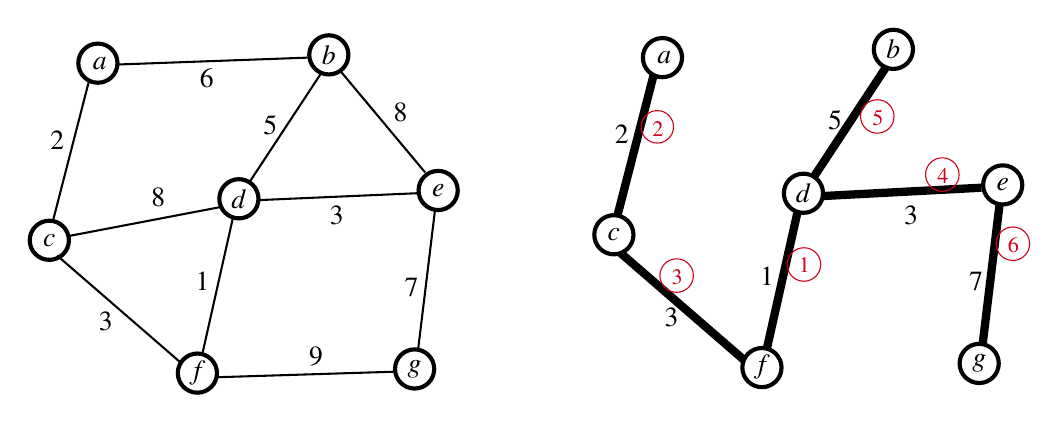
\begin{tikzpicture}[x=0.5pt,y=0.5pt,yscale=-1,xscale=1]
%uncomment if require: \path (0,294); %set diagram left start at 0, and has height of 294

%Straight Lines [id:da6859712806144006] 
\draw [color={rgb, 255:red, 0; green, 0; blue, 0 }  ,draw opacity=1 ][line width=0.75]    (237,42) -- (298,115) ;
%Straight Lines [id:da43828905709564314] 
\draw [color={rgb, 255:red, 0; green, 0; blue, 0 }  ,draw opacity=1 ][line width=0.75]    (147,263) -- (275,259) ;
%Straight Lines [id:da6385368954330931] 
\draw [color={rgb, 255:red, 0; green, 0; blue, 0 }  ,draw opacity=1 ][line width=0.75]    (32,175) -- (122,253) ;
%Straight Lines [id:da061278223687582845] 
\draw [color={rgb, 255:red, 0; green, 0; blue, 0 }  ,draw opacity=1 ][line width=0.75]    (40,161) -- (150,140) ;
%Straight Lines [id:da125058897644165] 
\draw [color={rgb, 255:red, 0; green, 0; blue, 0 }  ,draw opacity=1 ][line width=0.75]    (55,49) -- (29,150) ;
%Straight Lines [id:da7561477389708726] 
\draw [color={rgb, 255:red, 0; green, 0; blue, 0 }  ,draw opacity=1 ][line width=0.75]    (75,37) -- (213,32) ;
%Straight Lines [id:da8045438090716241] 
\draw [color={rgb, 255:red, 0; green, 0; blue, 0 }  ,draw opacity=1 ][line width=0.75]    (223,43) -- (171,122) ;
%Straight Lines [id:da7384444755679203] 
\draw [color={rgb, 255:red, 0; green, 0; blue, 0 }  ,draw opacity=1 ][line width=0.75]    (159,148) -- (137,246) ;
%Straight Lines [id:da7781378597799559] 
\draw [color={rgb, 255:red, 0; green, 0; blue, 0 }  ,draw opacity=1 ][line width=0.75]    (305,143) -- (293,242) ;
%Straight Lines [id:da6283012441188964] 
\draw [color={rgb, 255:red, 0; green, 0; blue, 0 }  ,draw opacity=1 ][line width=0.75]    (292,130) -- (177,135) ;
%Straight Lines [id:da8730022909148112] 
\draw [color={rgb, 255:red, 0; green, 0; blue, 0 }  ,draw opacity=1 ][line width=3]    (586,132) -- (700,126) ;
%Straight Lines [id:da5161692873874864] 
\draw [color={rgb, 255:red, 0; green, 0; blue, 0 }  ,draw opacity=1 ][line width=3]    (463,45) -- (437,146) ;
%Straight Lines [id:da4352724287531199] 
\draw [color={rgb, 255:red, 0; green, 0; blue, 0 }  ,draw opacity=1 ][line width=3]    (631,39) -- (579,118) ;
%Straight Lines [id:da4878171039675874] 
\draw [color={rgb, 255:red, 0; green, 0; blue, 0 }  ,draw opacity=1 ][line width=3]    (567,144) -- (545,242) ;
%Straight Lines [id:da9647292972064201] 
\draw [color={rgb, 255:red, 0; green, 0; blue, 0 }  ,draw opacity=1 ][line width=3]    (713,139) -- (701,238) ;
%Straight Lines [id:da358430115249718] 
\draw [color={rgb, 255:red, 0; green, 0; blue, 0 }  ,draw opacity=1 ][line width=3]    (439,173) -- (529,251) ;

% Text Node
\draw  [line width=1.5]   (307.38, 128) circle [x radius= 14.15, y radius= 14.15]   ;
\draw (307.38,128) node   [align=left] {$\displaystyle e$};
% Text Node
\draw  [line width=1.5]   (61.48, 36) circle [x radius= 14.15, y radius= 14.15]   ;
\draw (55.98,36) node [anchor=west] [inner sep=0.75pt]   [align=left] {$\displaystyle a$};
% Text Node
\draw  [line width=1.5]   (228.38, 30) circle [x radius= 14.15, y radius= 14.15]   ;
\draw (228.38,30) node   [align=left] {$\displaystyle b$};
% Text Node
\draw  [line width=1.5]   (26.38, 164) circle [x radius= 14.15, y radius= 14.15]   ;
\draw (26.38,164) node   [align=left] {$\displaystyle c$};
% Text Node
\draw  [line width=1.5]   (163.38, 134) circle [x radius= 14.15, y radius= 14.15]   ;
\draw (163.38,134) node   [align=left] {$\displaystyle d$};
% Text Node
\draw  [line width=1.5]   (133.38, 260) circle [x radius= 14.15, y radius= 14.15]   ;
\draw (133.38,260) node   [align=left] {$\displaystyle f$};
% Text Node
\draw  [line width=1.5]   (290.38, 257) circle [x radius= 14.15, y radius= 14.15]   ;
\draw (290.38,257) node   [align=left] {$\displaystyle g$};
% Text Node
\draw (25.24,83.06) node [anchor=north west][inner sep=0.75pt]   [align=left] {$\displaystyle 2$};
% Text Node
\draw (133.24,38.06) node [anchor=north west][inner sep=0.75pt]   [align=left] {$\displaystyle 6$};
% Text Node
\draw (227.24,137.06) node [anchor=north west][inner sep=0.75pt]   [align=left] {$\displaystyle 3$};
% Text Node
\draw (179.24,72.06) node [anchor=north west][inner sep=0.75pt]   [align=left] {$\displaystyle 5$};
% Text Node
\draw (98.24,124.06) node [anchor=north west][inner sep=0.75pt]   [align=left] {$\displaystyle 8$};
% Text Node
\draw (60.24,214.06) node [anchor=north west][inner sep=0.75pt]   [align=left] {$\displaystyle 3$};
% Text Node
\draw (130.24,185.06) node [anchor=north west][inner sep=0.75pt]   [align=left] {$\displaystyle 1$};
% Text Node
\draw (273.24,63.06) node [anchor=north west][inner sep=0.75pt]   [align=left] {$\displaystyle 8$};
% Text Node
\draw (212.24,239.06) node [anchor=north west][inner sep=0.75pt]   [align=left] {$\displaystyle 9$};
% Text Node
\draw (281.24,189) node [anchor=north west][inner sep=0.75pt]   [align=left] {$\displaystyle 7$};
% Text Node
\draw  [line width=1.5]   (715.38, 124) circle [x radius= 14.15, y radius= 14.15]   ;
\draw (715.38,124) node   [align=left] {$\displaystyle e$};
% Text Node
\draw  [line width=1.5]   (469.48, 32) circle [x radius= 14.15, y radius= 14.15]   ;
\draw (463.98,32) node [anchor=west] [inner sep=0.75pt]   [align=left] {$\displaystyle a$};
% Text Node
\draw  [line width=1.5]   (636.38, 26) circle [x radius= 14.15, y radius= 14.15]   ;
\draw (636.38,26) node   [align=left] {$\displaystyle b$};
% Text Node
\draw  [line width=1.5]   (434.38, 160) circle [x radius= 14.15, y radius= 14.15]   ;
\draw (434.38,160) node   [align=left] {$\displaystyle c$};
% Text Node
\draw  [line width=1.5]   (571.38, 130) circle [x radius= 14.15, y radius= 14.15]   ;
\draw (571.38,130) node   [align=left] {$\displaystyle d$};
% Text Node
\draw  [line width=1.5]   (541.38, 256) circle [x radius= 14.15, y radius= 14.15]   ;
\draw (541.38,256) node   [align=left] {$\displaystyle f$};
% Text Node
\draw  [line width=1.5]   (698.38, 253) circle [x radius= 14.15, y radius= 14.15]   ;
\draw (698.38,253) node   [align=left] {$\displaystyle g$};
% Text Node
\draw (433.24,79.06) node [anchor=north west][inner sep=0.75pt]   [align=left] {$\displaystyle 2$};
% Text Node
\draw (642.24,137.06) node [anchor=north west][inner sep=0.75pt]   [align=left] {$\displaystyle 3$};
% Text Node
\draw (587.24,68.06) node [anchor=north west][inner sep=0.75pt]   [align=left] {$\displaystyle 5$};
% Text Node
\draw (538.24,181.06) node [anchor=north west][inner sep=0.75pt]   [align=left] {$\displaystyle 1$};
% Text Node
\draw (689.24,185) node [anchor=north west][inner sep=0.75pt]   [align=left] {$\displaystyle 7$};
% Text Node
\draw  [color={rgb, 255:red, 208; green, 2; blue, 27 }  ,draw opacity=1 ]  (571.74, 181.5) circle [x radius= 12.1, y radius= 12.1]   ;
\draw (566.24,175) node [anchor=north west][inner sep=0.75pt]  [font=\footnotesize,color={rgb, 255:red, 208; green, 2; blue, 27 }  ,opacity=1 ] [align=left] {$\displaystyle 1$};
% Text Node
\draw  [color={rgb, 255:red, 208; green, 2; blue, 27 }  ,draw opacity=1 ]  (465.74, 82) circle [x radius= 11.72, y radius= 11.72]   ;
\draw (460.24,76) node [anchor=north west][inner sep=0.75pt]  [font=\footnotesize,color={rgb, 255:red, 208; green, 2; blue, 27 }  ,opacity=1 ] [align=left] {2};
% Text Node
\draw  [color={rgb, 255:red, 208; green, 2; blue, 27 }  ,draw opacity=1 ]  (624.74, 74.5) circle [x radius= 12.1, y radius= 12.1]   ;
\draw (619.24,68) node [anchor=north west][inner sep=0.75pt]  [font=\footnotesize,color={rgb, 255:red, 208; green, 2; blue, 27 }  ,opacity=1 ] [align=left] {$\displaystyle 5$};
% Text Node
\draw (469.24,211.06) node [anchor=north west][inner sep=0.75pt]   [align=left] {$\displaystyle 3$};
% Text Node
\draw  [color={rgb, 255:red, 208; green, 2; blue, 27 }  ,draw opacity=1 ]  (479.74, 189.5) circle [x radius= 12.1, y radius= 12.1]   ;
\draw (474.24,183) node [anchor=north west][inner sep=0.75pt]  [font=\footnotesize,color={rgb, 255:red, 208; green, 2; blue, 27 }  ,opacity=1 ] [align=left] {$\displaystyle 3$};
% Text Node
\draw  [color={rgb, 255:red, 208; green, 2; blue, 27 }  ,draw opacity=1 ]  (671.74, 116.5) circle [x radius= 12.1, y radius= 12.1]   ;
\draw (666.24,110) node [anchor=north west][inner sep=0.75pt]  [font=\footnotesize,color={rgb, 255:red, 208; green, 2; blue, 27 }  ,opacity=1 ] [align=left] {$\displaystyle 4$};
% Text Node
\draw  [color={rgb, 255:red, 208; green, 2; blue, 27 }  ,draw opacity=1 ]  (722.74, 166.5) circle [x radius= 12.1, y radius= 12.1]   ;
\draw (717.24,160) node [anchor=north west][inner sep=0.75pt]  [font=\footnotesize,color={rgb, 255:red, 208; green, 2; blue, 27 }  ,opacity=1 ] [align=left] {$\displaystyle 6$};


\end{tikzpicture}

}
\caption{Running Kruskal's algorithm. The cycled numbers give the order edges are picked.}
\label{fig:mst1}
\end{figure}

\subsection*{Prim's Algorithm}

Prim's algorithm combines the greedy strategy~(i.e., pick the smallest edge whenever possible)
and the 2nd way to construct a spanning tree~(i.e., pick $(|V|-1)$ edges that connects all vertices).
To connect all vertices, we can start from an \emph{arbitrary} vertex and iteratively
make it connected to all other vertices. As we need to use $(|V| - 1)$ edges to connect
to all other $(|V|-1)$ vertices, therefore every edge we pick needs to be connected to a
\emph{new} vertex.
Prim's algorithm can be summarized as: \emph{iteratively pick $(|V|-1)$ edges,
and in each iteration, pick the smallest edge that connects to a new vertex}.
We again use $E_1$ to store the picked edges.
We also use $S$ to store the vertices that have been connected.
The pseudo-code is given below.  See an example in Figure~\ref{fig:mst2}.

\begin{minipage}{0.8\textwidth}
	\aaA {8}{Algorithm Prim's~(graph $G = (V, E)$)}\xxx
	\aab {init $E_1 = \emptyset$;}\xxx
	\aab {init $S$ with an arbitrarily picked vertex;}\xxx
	\aaB {4}{for $k = 1 \to |V| - 1$}\xxx
	\aac {pick the smallest edge $e = (u,v)$ that connects to a new vertex~(i.e., $u\in S$ and $v\not\in S$);}\xxx
	\aac {$E_1 = E_1\cup\{e\}$;}\xxx
	\aac {$S = S\cup\{v\}$;}\xxx
	\aab {end for;}\xxx
	\aaa {end algorithm;}\xxx
\end{minipage}

\begin{figure}[h]
\centering{

\tikzset{every picture/.style={line width=0.75pt}} %set default line width to 0.75pt        

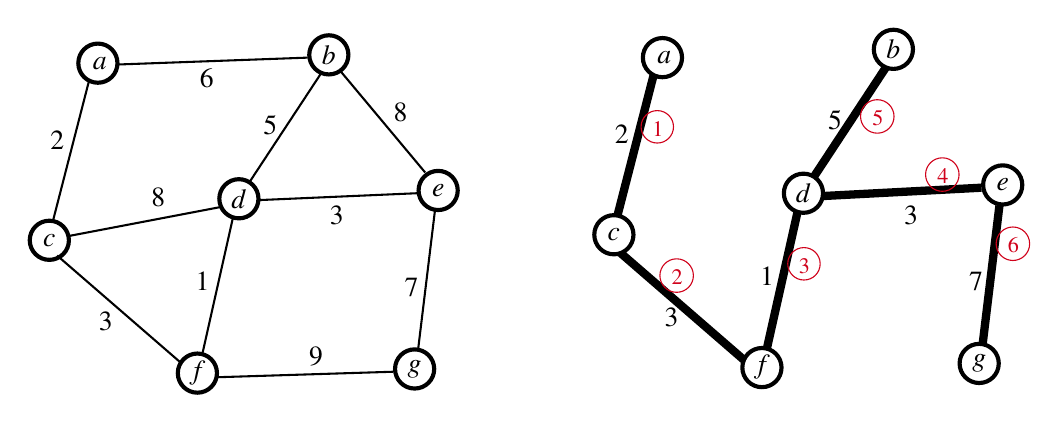
\begin{tikzpicture}[x=0.5pt,y=0.5pt,yscale=-1,xscale=1]
%uncomment if require: \path (0,294); %set diagram left start at 0, and has height of 294

%Straight Lines [id:da6859712806144006] 
\draw [color={rgb, 255:red, 0; green, 0; blue, 0 }  ,draw opacity=1 ][line width=0.75]    (237,42) -- (298,115) ;
%Straight Lines [id:da43828905709564314] 
\draw [color={rgb, 255:red, 0; green, 0; blue, 0 }  ,draw opacity=1 ][line width=0.75]    (147,263) -- (275,259) ;
%Straight Lines [id:da6385368954330931] 
\draw [color={rgb, 255:red, 0; green, 0; blue, 0 }  ,draw opacity=1 ][line width=0.75]    (32,175) -- (122,253) ;
%Straight Lines [id:da061278223687582845] 
\draw [color={rgb, 255:red, 0; green, 0; blue, 0 }  ,draw opacity=1 ][line width=0.75]    (40,161) -- (150,140) ;
%Straight Lines [id:da125058897644165] 
\draw [color={rgb, 255:red, 0; green, 0; blue, 0 }  ,draw opacity=1 ][line width=0.75]    (55,49) -- (29,150) ;
%Straight Lines [id:da7561477389708726] 
\draw [color={rgb, 255:red, 0; green, 0; blue, 0 }  ,draw opacity=1 ][line width=0.75]    (75,37) -- (213,32) ;
%Straight Lines [id:da8045438090716241] 
\draw [color={rgb, 255:red, 0; green, 0; blue, 0 }  ,draw opacity=1 ][line width=0.75]    (223,43) -- (171,122) ;
%Straight Lines [id:da7384444755679203] 
\draw [color={rgb, 255:red, 0; green, 0; blue, 0 }  ,draw opacity=1 ][line width=0.75]    (159,148) -- (137,246) ;
%Straight Lines [id:da7781378597799559] 
\draw [color={rgb, 255:red, 0; green, 0; blue, 0 }  ,draw opacity=1 ][line width=0.75]    (305,143) -- (293,242) ;
%Straight Lines [id:da6283012441188964] 
\draw [color={rgb, 255:red, 0; green, 0; blue, 0 }  ,draw opacity=1 ][line width=0.75]    (292,130) -- (177,135) ;
%Straight Lines [id:da8730022909148112] 
\draw [color={rgb, 255:red, 0; green, 0; blue, 0 }  ,draw opacity=1 ][line width=3]    (586,132) -- (700,126) ;
%Straight Lines [id:da5161692873874864] 
\draw [color={rgb, 255:red, 0; green, 0; blue, 0 }  ,draw opacity=1 ][line width=3]    (463,45) -- (437,146) ;
%Straight Lines [id:da4352724287531199] 
\draw [color={rgb, 255:red, 0; green, 0; blue, 0 }  ,draw opacity=1 ][line width=3]    (631,39) -- (579,118) ;
%Straight Lines [id:da4878171039675874] 
\draw [color={rgb, 255:red, 0; green, 0; blue, 0 }  ,draw opacity=1 ][line width=3]    (567,144) -- (545,242) ;
%Straight Lines [id:da9647292972064201] 
\draw [color={rgb, 255:red, 0; green, 0; blue, 0 }  ,draw opacity=1 ][line width=3]    (713,139) -- (701,238) ;
%Straight Lines [id:da358430115249718] 
\draw [color={rgb, 255:red, 0; green, 0; blue, 0 }  ,draw opacity=1 ][line width=3]    (439,173) -- (529,251) ;

% Text Node
\draw  [line width=1.5]   (307.38, 128) circle [x radius= 14.15, y radius= 14.15]   ;
\draw (307.38,128) node   [align=left] {$\displaystyle e$};
% Text Node
\draw  [line width=1.5]   (61.48, 36) circle [x radius= 14.15, y radius= 14.15]   ;
\draw (55.98,36) node [anchor=west] [inner sep=0.75pt]   [align=left] {$\displaystyle a$};
% Text Node
\draw  [line width=1.5]   (228.38, 30) circle [x radius= 14.15, y radius= 14.15]   ;
\draw (228.38,30) node   [align=left] {$\displaystyle b$};
% Text Node
\draw  [line width=1.5]   (26.38, 164) circle [x radius= 14.15, y radius= 14.15]   ;
\draw (26.38,164) node   [align=left] {$\displaystyle c$};
% Text Node
\draw  [line width=1.5]   (163.38, 134) circle [x radius= 14.15, y radius= 14.15]   ;
\draw (163.38,134) node   [align=left] {$\displaystyle d$};
% Text Node
\draw  [line width=1.5]   (133.38, 260) circle [x radius= 14.15, y radius= 14.15]   ;
\draw (133.38,260) node   [align=left] {$\displaystyle f$};
% Text Node
\draw  [line width=1.5]   (290.38, 257) circle [x radius= 14.15, y radius= 14.15]   ;
\draw (290.38,257) node   [align=left] {$\displaystyle g$};
% Text Node
\draw (25.24,83.06) node [anchor=north west][inner sep=0.75pt]   [align=left] {$\displaystyle 2$};
% Text Node
\draw (133.24,38.06) node [anchor=north west][inner sep=0.75pt]   [align=left] {$\displaystyle 6$};
% Text Node
\draw (227.24,137.06) node [anchor=north west][inner sep=0.75pt]   [align=left] {$\displaystyle 3$};
% Text Node
\draw (179.24,72.06) node [anchor=north west][inner sep=0.75pt]   [align=left] {$\displaystyle 5$};
% Text Node
\draw (98.24,124.06) node [anchor=north west][inner sep=0.75pt]   [align=left] {$\displaystyle 8$};
% Text Node
\draw (60.24,214.06) node [anchor=north west][inner sep=0.75pt]   [align=left] {$\displaystyle 3$};
% Text Node
\draw (130.24,185.06) node [anchor=north west][inner sep=0.75pt]   [align=left] {$\displaystyle 1$};
% Text Node
\draw (273.24,63.06) node [anchor=north west][inner sep=0.75pt]   [align=left] {$\displaystyle 8$};
% Text Node
\draw (212.24,239.06) node [anchor=north west][inner sep=0.75pt]   [align=left] {$\displaystyle 9$};
% Text Node
\draw (281.24,189) node [anchor=north west][inner sep=0.75pt]   [align=left] {$\displaystyle 7$};
% Text Node
\draw  [line width=1.5]   (715.38, 124) circle [x radius= 14.15, y radius= 14.15]   ;
\draw (715.38,124) node   [align=left] {$\displaystyle e$};
% Text Node
\draw  [line width=1.5]   (469.48, 32) circle [x radius= 14.15, y radius= 14.15]   ;
\draw (463.98,32) node [anchor=west] [inner sep=0.75pt]   [align=left] {$\displaystyle a$};
% Text Node
\draw  [line width=1.5]   (636.38, 26) circle [x radius= 14.15, y radius= 14.15]   ;
\draw (636.38,26) node   [align=left] {$\displaystyle b$};
% Text Node
\draw  [line width=1.5]   (434.38, 160) circle [x radius= 14.15, y radius= 14.15]   ;
\draw (434.38,160) node   [align=left] {$\displaystyle c$};
% Text Node
\draw  [line width=1.5]   (571.38, 130) circle [x radius= 14.15, y radius= 14.15]   ;
\draw (571.38,130) node   [align=left] {$\displaystyle d$};
% Text Node
\draw  [line width=1.5]   (541.38, 256) circle [x radius= 14.15, y radius= 14.15]   ;
\draw (541.38,256) node   [align=left] {$\displaystyle f$};
% Text Node
\draw  [line width=1.5]   (698.38, 253) circle [x radius= 14.15, y radius= 14.15]   ;
\draw (698.38,253) node   [align=left] {$\displaystyle g$};
% Text Node
\draw (433.24,79.06) node [anchor=north west][inner sep=0.75pt]   [align=left] {$\displaystyle 2$};
% Text Node
\draw (642.24,137.06) node [anchor=north west][inner sep=0.75pt]   [align=left] {$\displaystyle 3$};
% Text Node
\draw (587.24,68.06) node [anchor=north west][inner sep=0.75pt]   [align=left] {$\displaystyle 5$};
% Text Node
\draw (538.24,181.06) node [anchor=north west][inner sep=0.75pt]   [align=left] {$\displaystyle 1$};
% Text Node
\draw (689.24,185) node [anchor=north west][inner sep=0.75pt]   [align=left] {$\displaystyle 7$};
% Text Node
\draw  [color={rgb, 255:red, 208; green, 2; blue, 27 }  ,draw opacity=1 ]  (571.74, 181) circle [x radius= 11.72, y radius= 11.72]   ;
\draw (566.24,175) node [anchor=north west][inner sep=0.75pt]  [font=\footnotesize,color={rgb, 255:red, 208; green, 2; blue, 27 }  ,opacity=1 ] [align=left] {3};
% Text Node
\draw  [color={rgb, 255:red, 208; green, 2; blue, 27 }  ,draw opacity=1 ]  (465.74, 82) circle [x radius= 11.72, y radius= 11.72]   ;
\draw (460.24,76) node [anchor=north west][inner sep=0.75pt]  [font=\footnotesize,color={rgb, 255:red, 208; green, 2; blue, 27 }  ,opacity=1 ] [align=left] {1};
% Text Node
\draw  [color={rgb, 255:red, 208; green, 2; blue, 27 }  ,draw opacity=1 ]  (624.74, 74.5) circle [x radius= 12.1, y radius= 12.1]   ;
\draw (619.24,68) node [anchor=north west][inner sep=0.75pt]  [font=\footnotesize,color={rgb, 255:red, 208; green, 2; blue, 27 }  ,opacity=1 ] [align=left] {$\displaystyle 5$};
% Text Node
\draw (469.24,211.06) node [anchor=north west][inner sep=0.75pt]   [align=left] {$\displaystyle 3$};
% Text Node
\draw  [color={rgb, 255:red, 208; green, 2; blue, 27 }  ,draw opacity=1 ]  (479.74, 189.5) circle [x radius= 12.1, y radius= 12.1]   ;
\draw (474.24,183) node [anchor=north west][inner sep=0.75pt]  [font=\footnotesize,color={rgb, 255:red, 208; green, 2; blue, 27 }  ,opacity=1 ] [align=left] {$\displaystyle 2$};
% Text Node
\draw  [color={rgb, 255:red, 208; green, 2; blue, 27 }  ,draw opacity=1 ]  (671.74, 116.5) circle [x radius= 12.1, y radius= 12.1]   ;
\draw (666.24,110) node [anchor=north west][inner sep=0.75pt]  [font=\footnotesize,color={rgb, 255:red, 208; green, 2; blue, 27 }  ,opacity=1 ] [align=left] {$\displaystyle 4$};
% Text Node
\draw  [color={rgb, 255:red, 208; green, 2; blue, 27 }  ,draw opacity=1 ]  (722.74, 166.5) circle [x radius= 12.1, y radius= 12.1]   ;
\draw (717.24,160) node [anchor=north west][inner sep=0.75pt]  [font=\footnotesize,color={rgb, 255:red, 208; green, 2; blue, 27 }  ,opacity=1 ] [align=left] {$\displaystyle 6$};


\end{tikzpicture}

}
\caption{Running Prim's algorithm with $S$ being initialized as $\{a\}$. The cycled numbers give the order edges are picked.}
\label{fig:mst2}
\end{figure}


Again the above algorithm is a framework, as how to select the
smallest edge that connects to a new vertex is not specified. 
Later on we will use \emph{priority queue} to efficiently do that.
We also need to prove the correctness of the Prim's algorithm, i.e., it can always find
an MST; we will do that later on.


\subsection*{Cut and Cut-Edges}

In order to develop a key property that proves the correctness of both Kruskal's algorithm
and the Prim's algorithm, we first introduce the definition of \emph{cut} and \emph{cut-edges}.
Let $G = (V, E)$ be a graph. A \emph{cut} $C$, denoted as $C = (S, V\setminus S)$,
is a partition of $V$~(i.e., $S$ and $V\setminus S$ where $S\subset V$).
Let $C = (S, V\setminus S)$ be a cut of $G$, we define the \emph{cut-edges} w.r.t.\ $C$,
denoted as $E(C)$, as $E(C) := \{(u,v)\in E\mid u\in S, v\in V\setminus S\}$.
See examples in Figure~\ref{fig:cut}.  Note the difference of cut-edges
when applied to undirected graphs and directed graphs.

\begin{figure}[h]
\centering{

\tikzset{every picture/.style={line width=0.75pt}} %set default line width to 0.75pt        

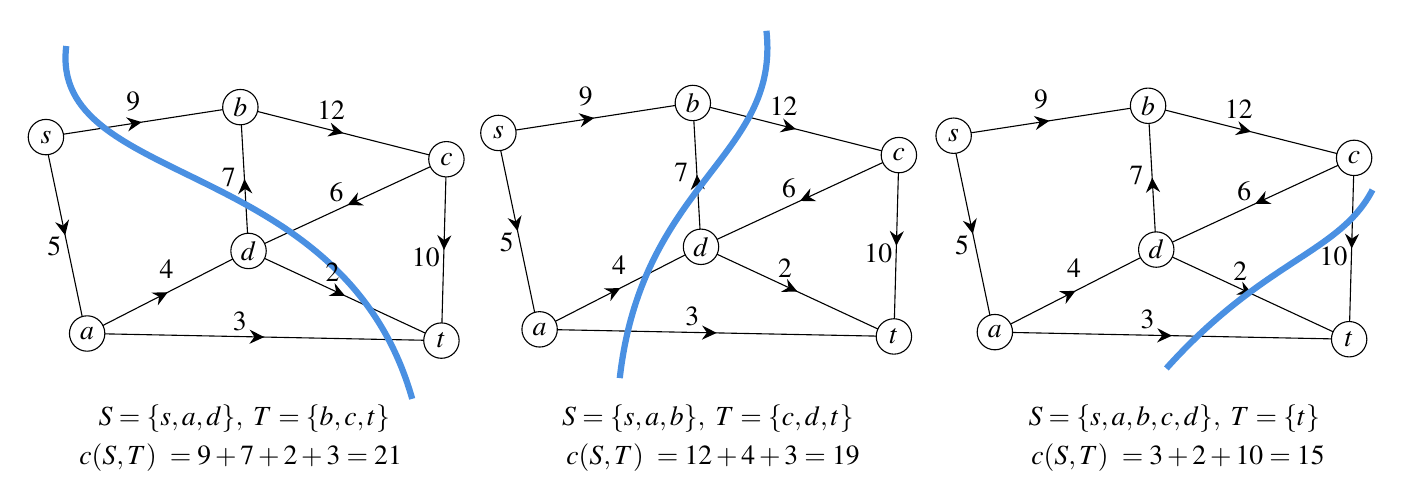
\begin{tikzpicture}[x=0.5pt,y=0.5pt,yscale=-1,xscale=1]
%uncomment if require: \path (0,338); %set diagram left start at 0, and has height of 338

%Straight Lines [id:da3853598268579197] 
\draw    (28.79,82.83) -- (169.31,61.18) ;
\draw [shift={(99.05,72)}, rotate = 531.24] [fill={rgb, 255:red, 0; green, 0; blue, 0 }  ][line width=0.08]  [draw opacity=0] (10.72,-5.15) -- (0,0) -- (10.72,5.15) -- (7.12,0) -- cycle    ;
%Straight Lines [id:da6958538828947681] 
\draw    (28.79,82.83) -- (58.58,224.77) ;
\draw [shift={(43.69,153.8)}, rotate = 258.15] [fill={rgb, 255:red, 0; green, 0; blue, 0 }  ][line width=0.08]  [draw opacity=0] (10.72,-5.15) -- (0,0) -- (10.72,5.15) -- (7.12,0) -- cycle    ;
%Straight Lines [id:da2980592918523626] 
\draw    (59.58,224.77) -- (315.62,229.9) ;
\draw [shift={(187.6,227.34)}, rotate = 181.15] [fill={rgb, 255:red, 0; green, 0; blue, 0 }  ][line width=0.08]  [draw opacity=0] (10.72,-5.15) -- (0,0) -- (10.72,5.15) -- (7.12,0) -- cycle    ;
%Straight Lines [id:da14604600957867897] 
\draw    (176.22,165.11) -- (315.62,229.9) ;
\draw [shift={(245.92,197.5)}, rotate = 204.92000000000002] [fill={rgb, 255:red, 0; green, 0; blue, 0 }  ][line width=0.08]  [draw opacity=0] (10.72,-5.15) -- (0,0) -- (10.72,5.15) -- (7.12,0) -- cycle    ;
%Straight Lines [id:da8640956582518242] 
\draw    (170.31,61.18) -- (176.22,165.11) ;
\draw [shift={(173.27,113.14)}, rotate = 86.75] [fill={rgb, 255:red, 0; green, 0; blue, 0 }  ][line width=0.08]  [draw opacity=0] (10.72,-5.15) -- (0,0) -- (10.72,5.15) -- (7.12,0) -- cycle    ;
%Straight Lines [id:da285469110869773] 
\draw    (170.31,61.18) -- (319.22,98.84) ;
\draw [shift={(244.76,80.01)}, rotate = 194.2] [fill={rgb, 255:red, 0; green, 0; blue, 0 }  ][line width=0.08]  [draw opacity=0] (10.72,-5.15) -- (0,0) -- (10.72,5.15) -- (7.12,0) -- cycle    ;
%Straight Lines [id:da8162300663234149] 
\draw    (319.22,98.84) -- (315.62,229.9) ;
\draw [shift={(317.42,164.37)}, rotate = 271.57] [fill={rgb, 255:red, 0; green, 0; blue, 0 }  ][line width=0.08]  [draw opacity=0] (10.72,-5.15) -- (0,0) -- (10.72,5.15) -- (7.12,0) -- cycle    ;
%Straight Lines [id:da5085854502811855] 
\draw    (319.22,98.84) -- (176.22,165.11) ;
\draw [shift={(247.72,131.98)}, rotate = 335.13] [fill={rgb, 255:red, 0; green, 0; blue, 0 }  ][line width=0.08]  [draw opacity=0] (10.72,-5.15) -- (0,0) -- (10.72,5.15) -- (7.12,0) -- cycle    ;
%Straight Lines [id:da4064365628912957] 
\draw    (176.22,165.11) -- (59.58,224.77) ;
\draw [shift={(117.9,194.94)}, rotate = 152.91] [fill={rgb, 255:red, 0; green, 0; blue, 0 }  ][line width=0.08]  [draw opacity=0] (10.72,-5.15) -- (0,0) -- (10.72,5.15) -- (7.12,0) -- cycle    ;
%Shape: Ellipse [id:dp651117123053256] 
\draw  [fill={rgb, 255:red, 255; green, 255; blue, 255 }  ,fill opacity=1 ] (17,82.83) .. controls (17,75.77) and (22.73,70.04) .. (29.79,70.04) .. controls (36.86,70.04) and (42.58,75.77) .. (42.58,82.83) .. controls (42.58,89.9) and (36.86,95.62) .. (29.79,95.62) .. controls (22.73,95.62) and (17,89.9) .. (17,82.83) -- cycle ;
%Shape: Ellipse [id:dp7399561756845123] 
\draw  [fill={rgb, 255:red, 255; green, 255; blue, 255 }  ,fill opacity=1 ] (157.52,61.18) .. controls (157.52,54.11) and (163.25,48.39) .. (170.31,48.39) .. controls (177.38,48.39) and (183.1,54.11) .. (183.1,61.18) .. controls (183.1,68.24) and (177.38,73.97) .. (170.31,73.97) .. controls (163.25,73.97) and (157.52,68.24) .. (157.52,61.18) -- cycle ;
%Shape: Ellipse [id:dp8268258265249401] 
\draw  [fill={rgb, 255:red, 255; green, 255; blue, 255 }  ,fill opacity=1 ] (306.43,98.84) .. controls (306.43,91.78) and (312.15,86.05) .. (319.22,86.05) .. controls (326.28,86.05) and (332.01,91.78) .. (332.01,98.84) .. controls (332.01,105.9) and (326.28,111.63) .. (319.22,111.63) .. controls (312.15,111.63) and (306.43,105.9) .. (306.43,98.84) -- cycle ;
%Shape: Ellipse [id:dp5421818862330341] 
\draw  [fill={rgb, 255:red, 255; green, 255; blue, 255 }  ,fill opacity=1 ] (163.43,165.11) .. controls (163.43,158.05) and (169.15,152.32) .. (176.22,152.32) .. controls (183.28,152.32) and (189.01,158.05) .. (189.01,165.11) .. controls (189.01,172.18) and (183.28,177.9) .. (176.22,177.9) .. controls (169.15,177.9) and (163.43,172.18) .. (163.43,165.11) -- cycle ;
%Shape: Ellipse [id:dp45600813719389455] 
\draw  [fill={rgb, 255:red, 255; green, 255; blue, 255 }  ,fill opacity=1 ] (46.79,224.77) .. controls (46.79,217.71) and (52.52,211.98) .. (59.58,211.98) .. controls (66.64,211.98) and (72.37,217.71) .. (72.37,224.77) .. controls (72.37,231.84) and (66.64,237.56) .. (59.58,237.56) .. controls (52.52,237.56) and (46.79,231.84) .. (46.79,224.77) -- cycle ;
%Shape: Ellipse [id:dp031187496945339066] 
\draw  [fill={rgb, 255:red, 255; green, 255; blue, 255 }  ,fill opacity=1 ] (302.83,229.9) .. controls (302.83,222.83) and (308.56,217.11) .. (315.62,217.11) .. controls (322.69,217.11) and (328.41,222.83) .. (328.41,229.9) .. controls (328.41,236.96) and (322.69,242.69) .. (315.62,242.69) .. controls (308.56,242.69) and (302.83,236.96) .. (302.83,229.9) -- cycle ;
%Straight Lines [id:da7435046067409884] 
\draw    (355.79,79.83) -- (496.31,58.18) ;
\draw [shift={(426.05,69)}, rotate = 531.24] [fill={rgb, 255:red, 0; green, 0; blue, 0 }  ][line width=0.08]  [draw opacity=0] (10.72,-5.15) -- (0,0) -- (10.72,5.15) -- (7.12,0) -- cycle    ;
%Straight Lines [id:da8387107518837462] 
\draw    (355.79,79.83) -- (385.58,221.77) ;
\draw [shift={(370.69,150.8)}, rotate = 258.15] [fill={rgb, 255:red, 0; green, 0; blue, 0 }  ][line width=0.08]  [draw opacity=0] (10.72,-5.15) -- (0,0) -- (10.72,5.15) -- (7.12,0) -- cycle    ;
%Straight Lines [id:da3219489964495771] 
\draw    (386.58,221.77) -- (642.62,226.9) ;
\draw [shift={(514.6,224.34)}, rotate = 181.15] [fill={rgb, 255:red, 0; green, 0; blue, 0 }  ][line width=0.08]  [draw opacity=0] (10.72,-5.15) -- (0,0) -- (10.72,5.15) -- (7.12,0) -- cycle    ;
%Straight Lines [id:da7100151765093478] 
\draw    (503.22,162.11) -- (642.62,226.9) ;
\draw [shift={(572.92,194.5)}, rotate = 204.92000000000002] [fill={rgb, 255:red, 0; green, 0; blue, 0 }  ][line width=0.08]  [draw opacity=0] (10.72,-5.15) -- (0,0) -- (10.72,5.15) -- (7.12,0) -- cycle    ;
%Straight Lines [id:da4338060480266903] 
\draw    (497.31,58.18) -- (503.22,162.11) ;
\draw [shift={(500.27,110.14)}, rotate = 86.75] [fill={rgb, 255:red, 0; green, 0; blue, 0 }  ][line width=0.08]  [draw opacity=0] (10.72,-5.15) -- (0,0) -- (10.72,5.15) -- (7.12,0) -- cycle    ;
%Straight Lines [id:da7182225488033221] 
\draw    (497.31,58.18) -- (646.22,95.84) ;
\draw [shift={(571.76,77.01)}, rotate = 194.2] [fill={rgb, 255:red, 0; green, 0; blue, 0 }  ][line width=0.08]  [draw opacity=0] (10.72,-5.15) -- (0,0) -- (10.72,5.15) -- (7.12,0) -- cycle    ;
%Straight Lines [id:da5940568426447731] 
\draw    (646.22,95.84) -- (642.62,226.9) ;
\draw [shift={(644.42,161.37)}, rotate = 271.57] [fill={rgb, 255:red, 0; green, 0; blue, 0 }  ][line width=0.08]  [draw opacity=0] (10.72,-5.15) -- (0,0) -- (10.72,5.15) -- (7.12,0) -- cycle    ;
%Straight Lines [id:da6584403815712339] 
\draw    (646.22,95.84) -- (503.22,162.11) ;
\draw [shift={(574.72,128.98)}, rotate = 335.13] [fill={rgb, 255:red, 0; green, 0; blue, 0 }  ][line width=0.08]  [draw opacity=0] (10.72,-5.15) -- (0,0) -- (10.72,5.15) -- (7.12,0) -- cycle    ;
%Straight Lines [id:da04611791534207066] 
\draw    (503.22,162.11) -- (386.58,221.77) ;
\draw [shift={(444.9,191.94)}, rotate = 152.91] [fill={rgb, 255:red, 0; green, 0; blue, 0 }  ][line width=0.08]  [draw opacity=0] (10.72,-5.15) -- (0,0) -- (10.72,5.15) -- (7.12,0) -- cycle    ;
%Shape: Ellipse [id:dp8684805017046724] 
\draw  [fill={rgb, 255:red, 255; green, 255; blue, 255 }  ,fill opacity=1 ] (344,79.83) .. controls (344,72.77) and (349.73,67.04) .. (356.79,67.04) .. controls (363.86,67.04) and (369.58,72.77) .. (369.58,79.83) .. controls (369.58,86.9) and (363.86,92.62) .. (356.79,92.62) .. controls (349.73,92.62) and (344,86.9) .. (344,79.83) -- cycle ;
%Shape: Ellipse [id:dp26598537007129874] 
\draw  [fill={rgb, 255:red, 255; green, 255; blue, 255 }  ,fill opacity=1 ] (484.52,58.18) .. controls (484.52,51.11) and (490.25,45.39) .. (497.31,45.39) .. controls (504.38,45.39) and (510.1,51.11) .. (510.1,58.18) .. controls (510.1,65.24) and (504.38,70.97) .. (497.31,70.97) .. controls (490.25,70.97) and (484.52,65.24) .. (484.52,58.18) -- cycle ;
%Shape: Ellipse [id:dp8446989445980774] 
\draw  [fill={rgb, 255:red, 255; green, 255; blue, 255 }  ,fill opacity=1 ] (633.43,95.84) .. controls (633.43,88.78) and (639.15,83.05) .. (646.22,83.05) .. controls (653.28,83.05) and (659.01,88.78) .. (659.01,95.84) .. controls (659.01,102.9) and (653.28,108.63) .. (646.22,108.63) .. controls (639.15,108.63) and (633.43,102.9) .. (633.43,95.84) -- cycle ;
%Shape: Ellipse [id:dp5784359228600563] 
\draw  [fill={rgb, 255:red, 255; green, 255; blue, 255 }  ,fill opacity=1 ] (490.43,162.11) .. controls (490.43,155.05) and (496.15,149.32) .. (503.22,149.32) .. controls (510.28,149.32) and (516.01,155.05) .. (516.01,162.11) .. controls (516.01,169.18) and (510.28,174.9) .. (503.22,174.9) .. controls (496.15,174.9) and (490.43,169.18) .. (490.43,162.11) -- cycle ;
%Shape: Ellipse [id:dp971944601404772] 
\draw  [fill={rgb, 255:red, 255; green, 255; blue, 255 }  ,fill opacity=1 ] (373.79,221.77) .. controls (373.79,214.71) and (379.52,208.98) .. (386.58,208.98) .. controls (393.64,208.98) and (399.37,214.71) .. (399.37,221.77) .. controls (399.37,228.84) and (393.64,234.56) .. (386.58,234.56) .. controls (379.52,234.56) and (373.79,228.84) .. (373.79,221.77) -- cycle ;
%Shape: Ellipse [id:dp1835030596812679] 
\draw  [fill={rgb, 255:red, 255; green, 255; blue, 255 }  ,fill opacity=1 ] (629.83,226.9) .. controls (629.83,219.83) and (635.56,214.11) .. (642.62,214.11) .. controls (649.69,214.11) and (655.41,219.83) .. (655.41,226.9) .. controls (655.41,233.96) and (649.69,239.69) .. (642.62,239.69) .. controls (635.56,239.69) and (629.83,233.96) .. (629.83,226.9) -- cycle ;
%Curve Lines [id:da2649473788057739] 
\draw [color={rgb, 255:red, 74; green, 144; blue, 226 }  ,draw opacity=1 ][line width=2.25]    (44.5,17) .. controls (31.5,120) and (244.5,95) .. (294.5,272) ;
%Curve Lines [id:da16888389279841676] 
\draw [color={rgb, 255:red, 74; green, 144; blue, 226 }  ,draw opacity=1 ][line width=2.25]    (550.5,6) .. controls (560.5,97) and (460.5,115) .. (444.5,257) ;
%Straight Lines [id:da23959710765930176] 
\draw    (684.79,81.83) -- (825.31,60.18) ;
\draw [shift={(755.05,71)}, rotate = 531.24] [fill={rgb, 255:red, 0; green, 0; blue, 0 }  ][line width=0.08]  [draw opacity=0] (10.72,-5.15) -- (0,0) -- (10.72,5.15) -- (7.12,0) -- cycle    ;
%Straight Lines [id:da6431206981927323] 
\draw    (684.79,81.83) -- (714.58,223.77) ;
\draw [shift={(699.69,152.8)}, rotate = 258.15] [fill={rgb, 255:red, 0; green, 0; blue, 0 }  ][line width=0.08]  [draw opacity=0] (10.72,-5.15) -- (0,0) -- (10.72,5.15) -- (7.12,0) -- cycle    ;
%Straight Lines [id:da5596554414836099] 
\draw    (715.58,223.77) -- (971.62,228.9) ;
\draw [shift={(843.6,226.34)}, rotate = 181.15] [fill={rgb, 255:red, 0; green, 0; blue, 0 }  ][line width=0.08]  [draw opacity=0] (10.72,-5.15) -- (0,0) -- (10.72,5.15) -- (7.12,0) -- cycle    ;
%Straight Lines [id:da8160720971935526] 
\draw    (832.22,164.11) -- (971.62,228.9) ;
\draw [shift={(901.92,196.5)}, rotate = 204.92000000000002] [fill={rgb, 255:red, 0; green, 0; blue, 0 }  ][line width=0.08]  [draw opacity=0] (10.72,-5.15) -- (0,0) -- (10.72,5.15) -- (7.12,0) -- cycle    ;
%Straight Lines [id:da3877819200248832] 
\draw    (826.31,60.18) -- (832.22,164.11) ;
\draw [shift={(829.27,112.14)}, rotate = 86.75] [fill={rgb, 255:red, 0; green, 0; blue, 0 }  ][line width=0.08]  [draw opacity=0] (10.72,-5.15) -- (0,0) -- (10.72,5.15) -- (7.12,0) -- cycle    ;
%Straight Lines [id:da057104792707504015] 
\draw    (826.31,60.18) -- (975.22,97.84) ;
\draw [shift={(900.76,79.01)}, rotate = 194.2] [fill={rgb, 255:red, 0; green, 0; blue, 0 }  ][line width=0.08]  [draw opacity=0] (10.72,-5.15) -- (0,0) -- (10.72,5.15) -- (7.12,0) -- cycle    ;
%Straight Lines [id:da14831136034761006] 
\draw    (975.22,97.84) -- (971.62,228.9) ;
\draw [shift={(973.42,163.37)}, rotate = 271.57] [fill={rgb, 255:red, 0; green, 0; blue, 0 }  ][line width=0.08]  [draw opacity=0] (10.72,-5.15) -- (0,0) -- (10.72,5.15) -- (7.12,0) -- cycle    ;
%Straight Lines [id:da2506057291921263] 
\draw    (975.22,97.84) -- (832.22,164.11) ;
\draw [shift={(903.72,130.98)}, rotate = 335.13] [fill={rgb, 255:red, 0; green, 0; blue, 0 }  ][line width=0.08]  [draw opacity=0] (10.72,-5.15) -- (0,0) -- (10.72,5.15) -- (7.12,0) -- cycle    ;
%Straight Lines [id:da7375159787579277] 
\draw    (832.22,164.11) -- (715.58,223.77) ;
\draw [shift={(773.9,193.94)}, rotate = 152.91] [fill={rgb, 255:red, 0; green, 0; blue, 0 }  ][line width=0.08]  [draw opacity=0] (10.72,-5.15) -- (0,0) -- (10.72,5.15) -- (7.12,0) -- cycle    ;
%Shape: Ellipse [id:dp7941672492891375] 
\draw  [fill={rgb, 255:red, 255; green, 255; blue, 255 }  ,fill opacity=1 ] (673,81.83) .. controls (673,74.77) and (678.73,69.04) .. (685.79,69.04) .. controls (692.86,69.04) and (698.58,74.77) .. (698.58,81.83) .. controls (698.58,88.9) and (692.86,94.62) .. (685.79,94.62) .. controls (678.73,94.62) and (673,88.9) .. (673,81.83) -- cycle ;
%Shape: Ellipse [id:dp3757660056746118] 
\draw  [fill={rgb, 255:red, 255; green, 255; blue, 255 }  ,fill opacity=1 ] (813.52,60.18) .. controls (813.52,53.11) and (819.25,47.39) .. (826.31,47.39) .. controls (833.38,47.39) and (839.1,53.11) .. (839.1,60.18) .. controls (839.1,67.24) and (833.38,72.97) .. (826.31,72.97) .. controls (819.25,72.97) and (813.52,67.24) .. (813.52,60.18) -- cycle ;
%Shape: Ellipse [id:dp9316219699822907] 
\draw  [fill={rgb, 255:red, 255; green, 255; blue, 255 }  ,fill opacity=1 ] (962.43,97.84) .. controls (962.43,90.78) and (968.15,85.05) .. (975.22,85.05) .. controls (982.28,85.05) and (988.01,90.78) .. (988.01,97.84) .. controls (988.01,104.9) and (982.28,110.63) .. (975.22,110.63) .. controls (968.15,110.63) and (962.43,104.9) .. (962.43,97.84) -- cycle ;
%Shape: Ellipse [id:dp2713572714021609] 
\draw  [fill={rgb, 255:red, 255; green, 255; blue, 255 }  ,fill opacity=1 ] (819.43,164.11) .. controls (819.43,157.05) and (825.15,151.32) .. (832.22,151.32) .. controls (839.28,151.32) and (845.01,157.05) .. (845.01,164.11) .. controls (845.01,171.18) and (839.28,176.9) .. (832.22,176.9) .. controls (825.15,176.9) and (819.43,171.18) .. (819.43,164.11) -- cycle ;
%Shape: Ellipse [id:dp8303944409855877] 
\draw  [fill={rgb, 255:red, 255; green, 255; blue, 255 }  ,fill opacity=1 ] (702.79,223.77) .. controls (702.79,216.71) and (708.52,210.98) .. (715.58,210.98) .. controls (722.64,210.98) and (728.37,216.71) .. (728.37,223.77) .. controls (728.37,230.84) and (722.64,236.56) .. (715.58,236.56) .. controls (708.52,236.56) and (702.79,230.84) .. (702.79,223.77) -- cycle ;
%Shape: Ellipse [id:dp3672414292204079] 
\draw  [fill={rgb, 255:red, 255; green, 255; blue, 255 }  ,fill opacity=1 ] (958.83,228.9) .. controls (958.83,221.83) and (964.56,216.11) .. (971.62,216.11) .. controls (978.69,216.11) and (984.41,221.83) .. (984.41,228.9) .. controls (984.41,235.96) and (978.69,241.69) .. (971.62,241.69) .. controls (964.56,241.69) and (958.83,235.96) .. (958.83,228.9) -- cycle ;
%Curve Lines [id:da42045420214553086] 
\draw [color={rgb, 255:red, 74; green, 144; blue, 226 }  ,draw opacity=1 ][line width=2.25]    (988.5,121) .. controls (964.5,167) and (910.5,171) .. (839.5,250) ;

% Text Node
\draw (29.79,82.83) node   [align=left] {$\displaystyle s$};
% Text Node
\draw (170.31,61.18) node   [align=left] {$\displaystyle b$};
% Text Node
\draw (319.22,98.84) node   [align=left] {$\displaystyle c$};
% Text Node
\draw (176.22,165.11) node   [align=left] {$\displaystyle d$};
% Text Node
\draw (59.58,224.77) node   [align=left] {$\displaystyle a$};
% Text Node
\draw (315.62,229.9) node   [align=left] {$\displaystyle t$};
% Text Node
\draw (29,153) node [anchor=north west][inner sep=0.75pt]   [align=left] {$\displaystyle 5$};
% Text Node
\draw (110,170) node [anchor=north west][inner sep=0.75pt]   [align=left] {$\displaystyle 4$};
% Text Node
\draw (86,48) node [anchor=north west][inner sep=0.75pt]   [align=left] {$\displaystyle 9$};
% Text Node
\draw (233,114) node [anchor=north west][inner sep=0.75pt]   [align=left] {$\displaystyle 6$};
% Text Node
\draw (155,103) node [anchor=north west][inner sep=0.75pt]   [align=left] {$\displaystyle 7$};
% Text Node
\draw (230,172) node [anchor=north west][inner sep=0.75pt]   [align=left] {$\displaystyle 2$};
% Text Node
\draw (292.42,161.37) node [anchor=north west][inner sep=0.75pt]   [align=left] {$\displaystyle 10$};
% Text Node
\draw (224,55) node [anchor=north west][inner sep=0.75pt]   [align=left] {$\displaystyle 12$};
% Text Node
\draw (163,207) node [anchor=north west][inner sep=0.75pt]   [align=left] {$\displaystyle 3$};
% Text Node
\draw (356.79,79.83) node   [align=left] {$\displaystyle s$};
% Text Node
\draw (497.31,58.18) node   [align=left] {$\displaystyle b$};
% Text Node
\draw (646.22,95.84) node   [align=left] {$\displaystyle c$};
% Text Node
\draw (503.22,162.11) node   [align=left] {$\displaystyle d$};
% Text Node
\draw (386.58,221.77) node   [align=left] {$\displaystyle a$};
% Text Node
\draw (642.62,226.9) node   [align=left] {$\displaystyle t$};
% Text Node
\draw (356,150) node [anchor=north west][inner sep=0.75pt]   [align=left] {$\displaystyle 5$};
% Text Node
\draw (437,167) node [anchor=north west][inner sep=0.75pt]   [align=left] {$\displaystyle 4$};
% Text Node
\draw (413,45) node [anchor=north west][inner sep=0.75pt]   [align=left] {$\displaystyle 9$};
% Text Node
\draw (560,111) node [anchor=north west][inner sep=0.75pt]   [align=left] {$\displaystyle 6$};
% Text Node
\draw (482,100) node [anchor=north west][inner sep=0.75pt]   [align=left] {$\displaystyle 7$};
% Text Node
\draw (557,169) node [anchor=north west][inner sep=0.75pt]   [align=left] {$\displaystyle 2$};
% Text Node
\draw (619.42,158.37) node [anchor=north west][inner sep=0.75pt]   [align=left] {$\displaystyle 10$};
% Text Node
\draw (551,52) node [anchor=north west][inner sep=0.75pt]   [align=left] {$\displaystyle 12$};
% Text Node
\draw (490,204) node [anchor=north west][inner sep=0.75pt]   [align=left] {$\displaystyle 3$};
% Text Node
\draw (52,302.5) node [anchor=north west][inner sep=0.75pt]   [align=left] {$\displaystyle c( S,T) \ =9+7+2+3=21$};
% Text Node
\draw (404,302.5) node [anchor=north west][inner sep=0.75pt]   [align=left] {$\displaystyle c( S,T) \ =12+4+3=19$};
% Text Node
\draw (685.79,81.83) node   [align=left] {$\displaystyle s$};
% Text Node
\draw (826.31,60.18) node   [align=left] {$\displaystyle b$};
% Text Node
\draw (975.22,97.84) node   [align=left] {$\displaystyle c$};
% Text Node
\draw (832.22,164.11) node   [align=left] {$\displaystyle d$};
% Text Node
\draw (715.58,223.77) node   [align=left] {$\displaystyle a$};
% Text Node
\draw (971.62,228.9) node   [align=left] {$\displaystyle t$};
% Text Node
\draw (685,152) node [anchor=north west][inner sep=0.75pt]   [align=left] {$\displaystyle 5$};
% Text Node
\draw (766,169) node [anchor=north west][inner sep=0.75pt]   [align=left] {$\displaystyle 4$};
% Text Node
\draw (742,47) node [anchor=north west][inner sep=0.75pt]   [align=left] {$\displaystyle 9$};
% Text Node
\draw (889,113) node [anchor=north west][inner sep=0.75pt]   [align=left] {$\displaystyle 6$};
% Text Node
\draw (811,102) node [anchor=north west][inner sep=0.75pt]   [align=left] {$\displaystyle 7$};
% Text Node
\draw (886,171) node [anchor=north west][inner sep=0.75pt]   [align=left] {$\displaystyle 2$};
% Text Node
\draw (948.42,160.37) node [anchor=north west][inner sep=0.75pt]   [align=left] {$\displaystyle 10$};
% Text Node
\draw (880,54) node [anchor=north west][inner sep=0.75pt]   [align=left] {$\displaystyle 12$};
% Text Node
\draw (819,206) node [anchor=north west][inner sep=0.75pt]   [align=left] {$\displaystyle 3$};
% Text Node
\draw (740,302.5) node [anchor=north west][inner sep=0.75pt]   [align=left] {$\displaystyle c( S,T) \ =3+2+10=15$};
% Text Node
\draw (66,274.5) node [anchor=north west][inner sep=0.75pt]   [align=left] {$\displaystyle S=\{s,a,d\} ,\ T=\{b,c,t\}$};
% Text Node
\draw (401,274.5) node [anchor=north west][inner sep=0.75pt]   [align=left] {$\displaystyle S=\{s,a,b\} ,\ T=\{c,d,t\}$};
% Text Node
\draw (738,274.5) node [anchor=north west][inner sep=0.75pt]   [align=left] {$\displaystyle S=\{s,a,b,c,d\} ,\ T=\{t\}$};


\end{tikzpicture}

}
\caption{Cut and cut-edges on an undirected graph~(left) and on a directed graph~(right).
Cut-edges are highlighted with bold edges.}
\label{fig:cut}
\end{figure}

\end{document}
